
\begin{frame}[t]{Die Messbrücke - Arbeitspunktanalyse}  
    
    
    Die Grundlage für unsere Messbruecke bildet eine einfache Brückenschaltung. 
    Zur Wiederholung findet ihr unten den Schaltplan sowie die Formel zur Berechnung
    der Brueckenspannung. $V_{AB}$.

    
    \begin{table}[h!]
        \begin{tabular}{p{5cm} p{5cm}}
          \begin{minipage}{.5\textwidth}
            \begin{figure}
              \scalebox{0.6}{
            \centering
            \begin{circuitikz}
              \ctikzset{bipoles/thickness=1}
              \ctikzset{bipoles/length=.6cm}
              \draw
              (0,0) to [short, *-] (4,0)
              (0,0) to [V, l_=$V_{1}$] (0,-4)
              (2,0) to (2,-0.5) 
              (4,0) to (4,-0.5) 
              (2,-0.5) to [R, l_=$R_{1}$] (2,-1.5) 
              (2,-2.5) to [R, l_=$R_{2}$] (2,-3.5) 
              (2,-1.5) to (2,-2.5) 
              (2,-2) to [short,*-o] (2.25,-2) node[right]{$V_{a}$}
              (4,-1.5) to (4,-2.5) 
              (4,-2) to [short,*-o] (4.25,-2) node[right]{$V_{b}$}
              (4,-0.5) to [R, l_=$R_{3}$] (4,-1.5) 
              (4,-2.5) to [R, l_=$R_{4}$] (4,-3.5) 
              (2,-3.5) to (2,-4) 
              (4,-3.5) to (4,-4) 
              (0,-4) node[ground]{}
              (2,-4) node[ground]{}
              (4,-4) node[ground]{}
              ;
              \end{circuitikz} 
              }
              
          \end{figure}
          \end{minipage} 
          & 

        \begin{spacing}{0.9} \begin{tiny}
          \begin{minipage}{.5\textwidth}
          \begin{equation}
            V_{AB}=\frac{R_2R_3-R_4R_1}{(R_1+R_2)(R_3+R_4)}V_{1}
            \end{equation}
          \end{minipage} 
        \end{tiny} \end{spacing}
        \end{tabular}
      
      \end{table}

\end{frame}

    

\begin{frame}[t]{Die Messbrücke - Arbeitspunktanalyse} 
    
    \begin{spacing}{0.9} \begin{tiny}
    \begin{table}[h!]
      \begin{tabular}{p{3cm} p{7cm}}
        \hline
        \textbf{Simulation} & \\
        \hline \\
        \begin{minipage}{.3\textwidth}
         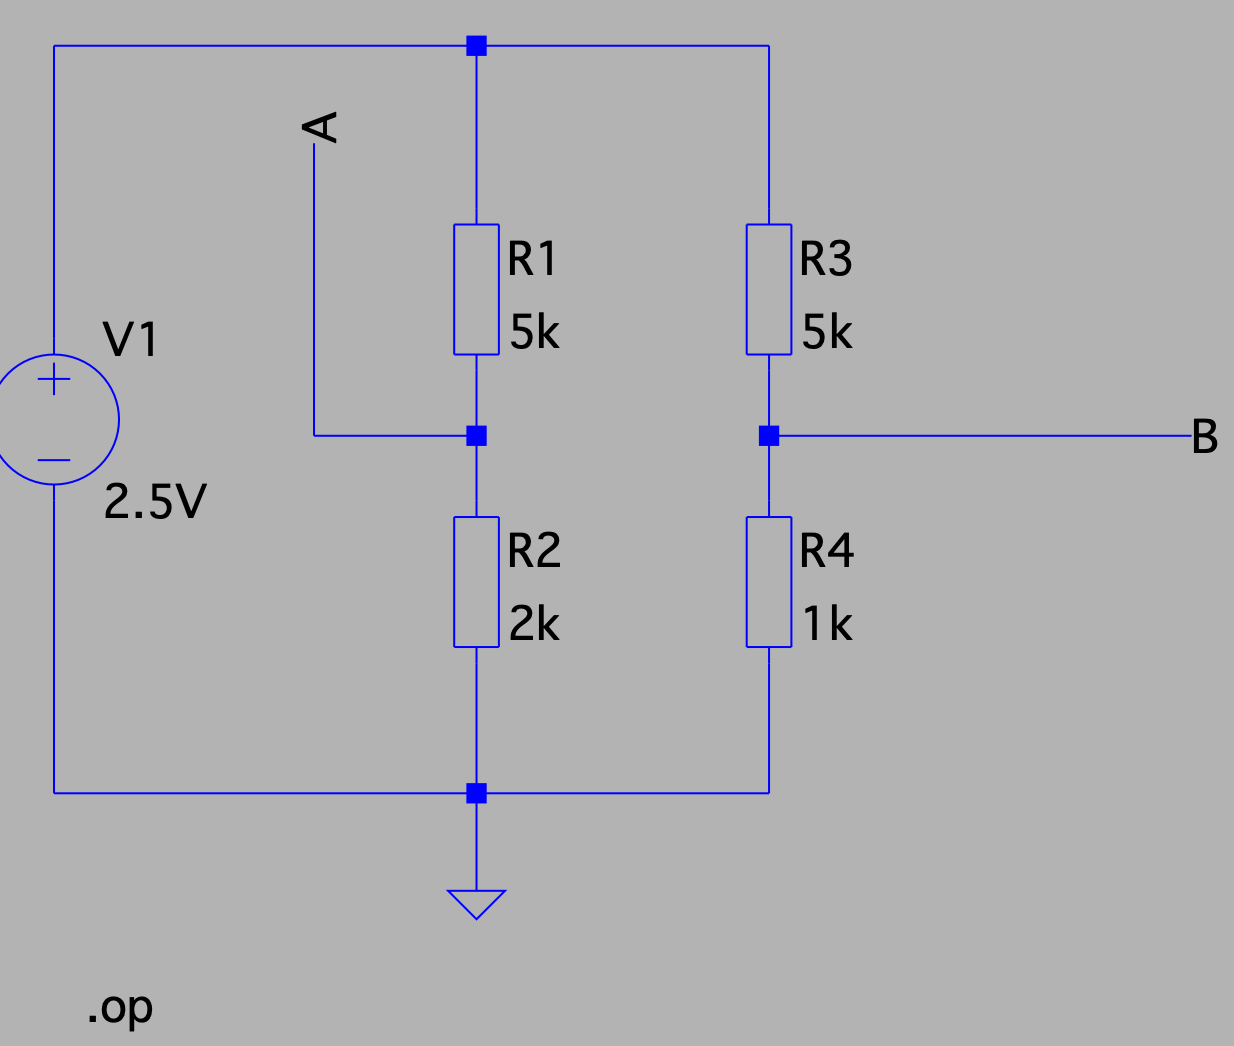
\includegraphics[width=\linewidth]{pictures/bridge_op_2.png}
       \end{minipage} 
       & 
       \begin{minipage}{.7\textwidth}
       \begin{itemize}
         \item Ihr baut die Brueckenschaltung entsprechend auf und verdrahtet Sie
         \item Wir wählen eine neue Analyseart, die Arbeitspunktanalyse \newline(.op == operation point)
         \item Ihr fügt .op als spice-Direktive hinzu \newline(oder wählt im simulation cmd DC Bias Point)
         \item Ihr klickt auf 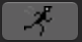
\includegraphics[scale=0.3]{pictures/run.png} (run)
       \end{itemize}
       \end{minipage} 
       \\
       &\\
       \hline
       \textbf{Exkurs zur Netzliste} & \\
       \hline \\
       \begin{minipage}{.3\textwidth}
        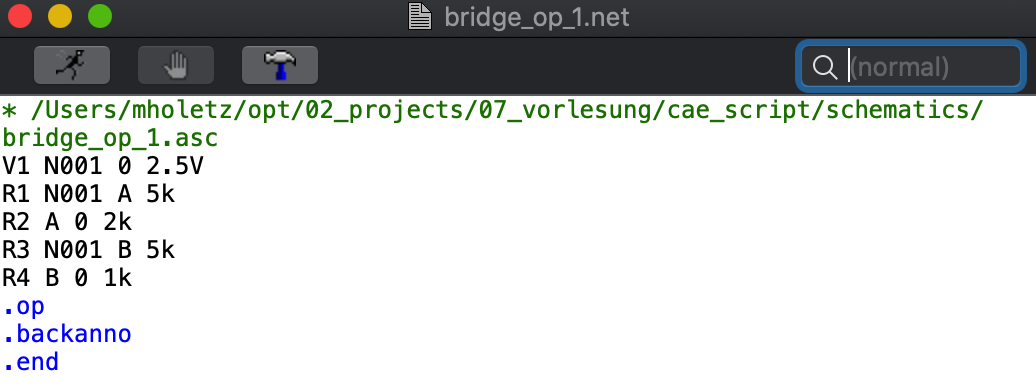
\includegraphics[width=\linewidth]{pictures/netlist.png}\newline
        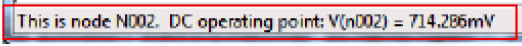
\includegraphics[width=\linewidth]{pictures/knotenname.png}
      \end{minipage} 
      & 
      \begin{minipage}{.7\textwidth}
      
      \begin{itemize}
        \item Der Spice Algorithmus mit einer Netzliste. 
        \item Jeder Knoten im Schaltplan erhält einen Namen. 
        \item Ihr könnt euch diese Netzliste per\newline rechtem Mausklick $->$ View $->$ SPICE Netlist anzeigen lassen. 
        \item Die Masse hat immer den Knotennamen \textbf{0}
        \item Wird ein Knoten \textbf{nicht explizit} mit einem \textbf{Label (F4)} versehen, numeriert LTspice sie aufsteigend durch (N001, N002, \dots)
        \item Weiterhin folgt eine Reihe in der Netzliste dem Schema\newline $<$Bauteil$>$ $<$Knoten1$>$ $<$Knoten2$>$ $<$Bauteilwert$>$
        \item z.B. Widerstand R2 geht von Knoten \textbf{A} (wir haben ein Label vergeben) zur Knoten \textbf{0} (Masse)   
        \item Wenn ihr mit der Maus über einen Knoten fahrt, wird euch unten links der Name des Knotens angezeigt.
      \end{itemize}
      \end{minipage} 
      \\
      \end{tabular}
    \end{table}
  \end{tiny} \end{spacing}
  

     \end{frame}

     \begin{frame}[t]{Die Messbrücke - Arbeitspunktanalyse} 
    
      \begin{spacing}{0.9} \begin{tiny}
      \begin{table}[h!]
        \begin{tabular}{p{3cm} p{7cm}}
         \hline
         \textbf{Analyse der Spannungswerte} & \\
         \hline \\
         \begin{minipage}{.3\textwidth}
          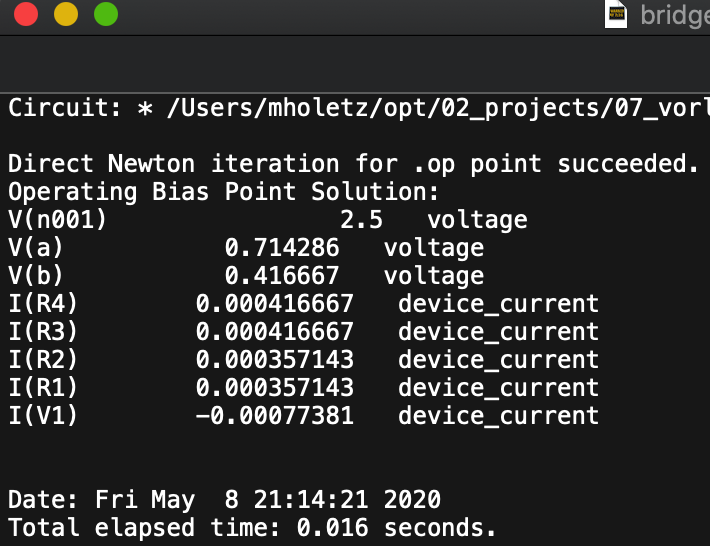
\includegraphics[width=\linewidth]{pictures/log_1.png}
        \end{minipage} 
        & 
        \begin{minipage}{.7\textwidth}
        
        Um die Spannungswerte abzulesen habt mehrere Möglichkeiten.
        \begin{itemize}
          \item Ihr könnt euch den log anzeigen lassen - er sollte direkt bei Start der Analyse erscheinen
          \item Ihr könnt \textbf{nach der Simulation} den gewünschten Knoten \textbf{zweimal} anklicken
          \item \textbf{V(KNOTENNAME)} beschreib das Potential an einem Knoten
          \item \textbf{I(BAUTEILNAME)} beschreibt den Strom durch ein Bauteil hindurch
          \item Per rechtem Mausklick auf einen Wert, öffnet sich ein Dialog über den ihr den Wert frei wählen könnt.
        \end{itemize}
        \end{minipage} 
        \\
        &\\
        \begin{minipage}{.3\textwidth}
         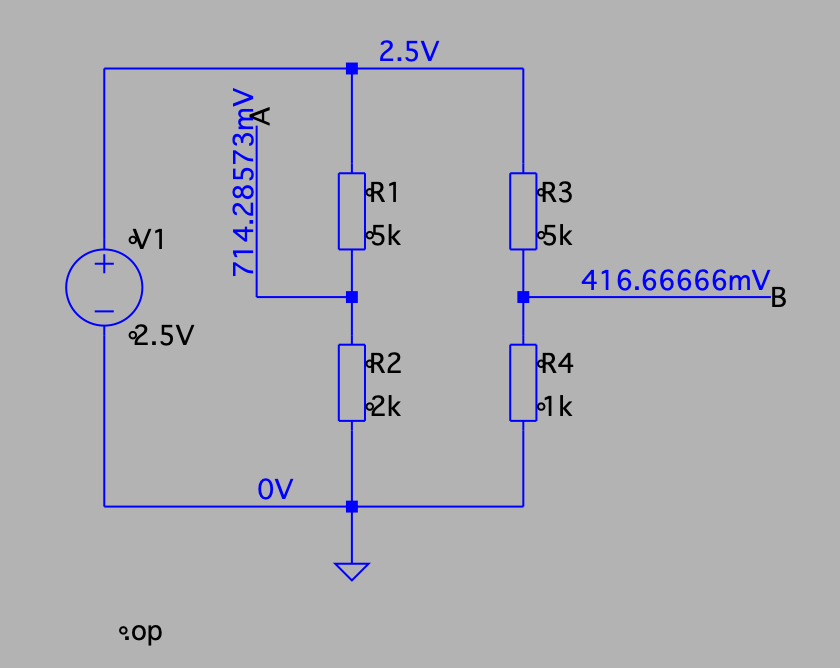
\includegraphics[width=\linewidth]{pictures/bridge_op_1.png}
       \end{minipage} 
       & 
       \begin{minipage}{.7\textwidth}
          Unter Verwendung der Potentiale und Ströme könnt ihr auch Formeln wie z.B. die Verlustleistung über einem Bauteil
          anzeigen. Per rechtem Mausklick auf einen Knotenspannungswert kommt ihr in das Display Data Menü.
          \begin{figure}
            \centering
            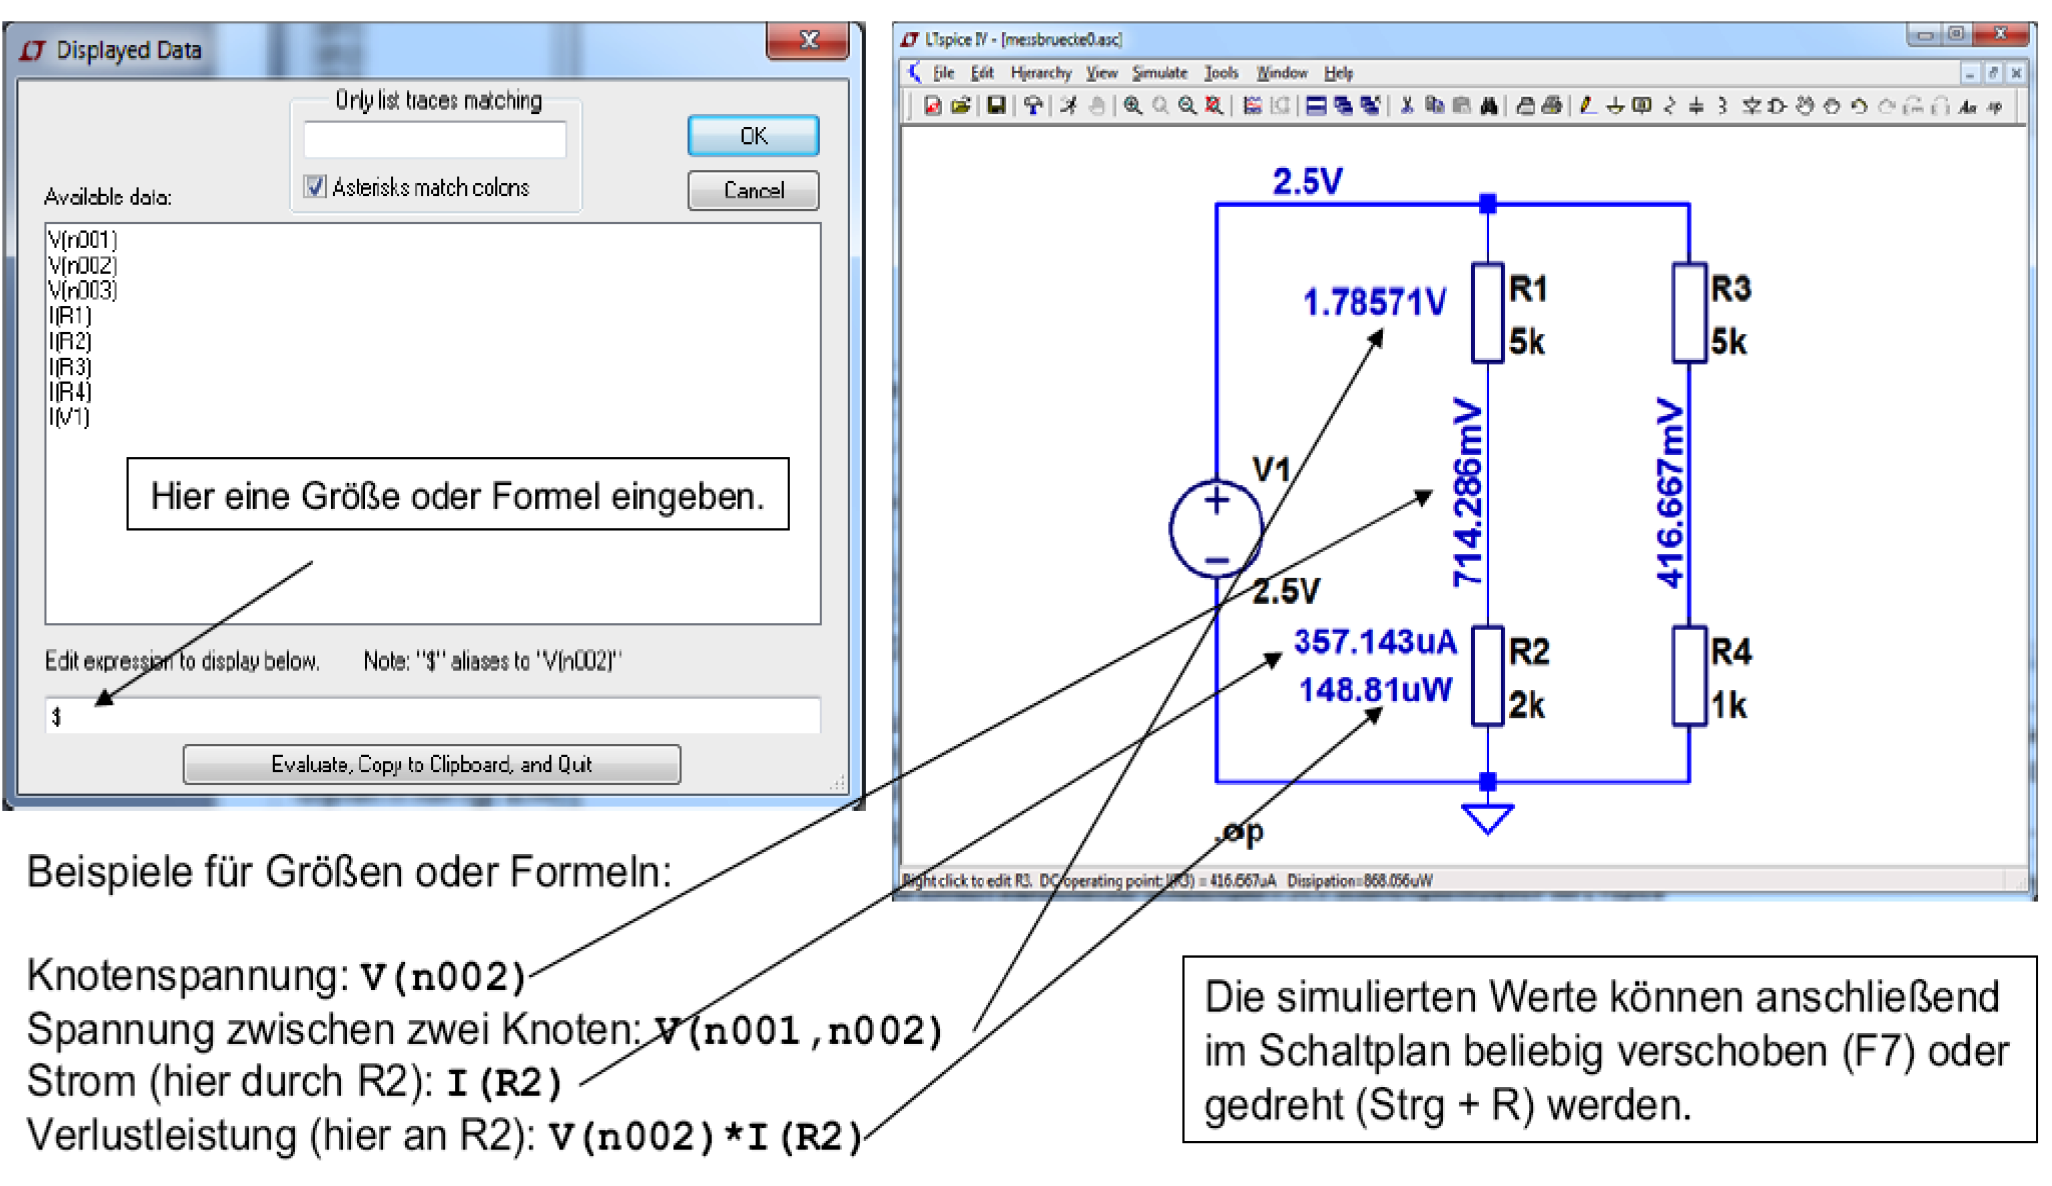
\includegraphics[width=0.8\linewidth]{pictures/manipulation.png}
          \end{figure}
       \end{minipage} 
       \\
        \end{tabular}
      \end{table}
    \end{tiny} \end{spacing}
    
  
       \end{frame}

